% This is the O7.tex LaTeX file
% Copyright 2010, Astronomical Society of the Pacific Conference Series

\documentclass[11pt,twoside]{article}
\usepackage{asp2010}

\resetcounters
\bibliographystyle{asp2010}
\markboth{Seo-Won Chang and Yong-Ik Byun}{Seo-Won Chang and Yong-Ik Byun}

\begin{document}

\title{Improvement of Time-Series Photometry based on Multi-Aperture
Indexing and Spatiotemporal de-trending}
\author{Seo-Won Chang and Yong-Ik Byun}
\affil{Department of Astronomy and University Observatory, Yonsei University, Seoul, Korea}

\begin{abstract}
High precision time-series photometry is often very difficult with ground-based surveys of large field of view.  Occasional failures of photometry due to contaminations, non-uniform cloud passages, and subtle PSF variations across the field are the major causes.  We developed a new photometry algorithm based on multi-aperture measurements and indexed aperture correction followed by spatio-temporal de-trending process.  This turns out to be a powerful method to improve overall photometric accuracy without the need to throw out many outlying data points.  The performance of our new method is demonstrated with MMT survey of M37 and HAT-South survey data.  The de-trending alone is also a very useful tool in removing systematics from light curves, as we demonstrate with a subset of light curves from LINEAR database.  Our method removes serious systematic variations that are shared by light curves of nearby stars, while true variabilities are preserved.  This greatly improves the usefulness of archived light curve data.
\end{abstract}


\section{High-precision Ground-based Photometry : Why and How}
New horizons in astronomical knowledge have often been preceded by improvement in methods of measurement or analysis.  For {\itshape wide-field} time-series data, much greater attention has recently been given to the data accuracy issue because we are now looking for very small photometric signatures (e.g., transiting exo-planets or stellar micro variability).  Another key issue in wide-field time-series photometry is the removal of temporal systematics (e.g., cloud passages, PSF variations, or instrumental artifacts).  These systematics make it difficult to identify and characterize low-amplitude variabilities.  We can overcome this difficulty with an adequate data analysis algorithm.  In this paper, we present and demonstrate the success of a new photometry procedure applied to the recalibration of three independent sets of archival survey data (MMT/Megacam, HAT-South, and LINEAR).

\subsection{Multi-aperture indexing photometry}
The aperture photometry with multiple apertures is an efficient way to determine the optimum aperture size that gives the maximum S/N for a flux measurement.  According to the CCD equation, the maximum S/N is not necessarily at the same aperture for all sources, and it can be obtained from a relatively small aperture \citep{how89}.

In practice, some stars may not be measurable in the optimal aperture in which the measured flux within the aperture area is contaminated by unwanted artifacts (e.g., cosmic rays, moving objects, bad pixels, or the effects of the nearby blended sources).  The data points with symptoms of artifacts tend to increase the rms scatter of the light curves, and thus are inevitably removed from the photometry table.  However, such stars often can be reliably measured through the smaller apertures which are not contaminated.  This also indicates that we may use the variation in enclosed flux profile through a series of apertures to identify and avoid the impact of contaminations.

We explain the concept of multi-aperture indexing and how it works with simple examples.  In the case of isolated objects, the average magnitude difference between a pair of apertures yields a precise determination of the total magnitude.  This flux correction method (i.e., growth-curve method) gives nearly the same brightness within the measurement uncertainties, while for the contaminated objects, aperture corrected magnitude deviates from its reference magnitude.    Here are the main points of the indexing process: \begin{itemize}
\item{We use the RMS of aperture correction as a criterion whether aperture corrected magnitude at a given aperture may or may not deviated from the reference magnitude.}

\item{The expected RMS value depends on the chosen magnitude interval.  To address this problem, we grouped all stars in a given field according to their brightness and then estimate RMS values for aperture corrections for each magnitude group.}

\item{In order to avoid over-estimation of the RMS value, we inspect member stars in each group to remove outliers using an iterative $\sigma$-clipping algorithm, and then determine the RMS model for each group.}

\item{For a given star, we compare differential magnitudes between apertures (=$m_{ref}-m_{ap}$) with mean trends for stars of similar brightness, and index the difference.  The index distribution guides us to choose whether to throw out or to replace some photometric measurements by aperture correction terms shared by other stars.}
\end{itemize}

\begin{figure}[!ht]
\begin{center}
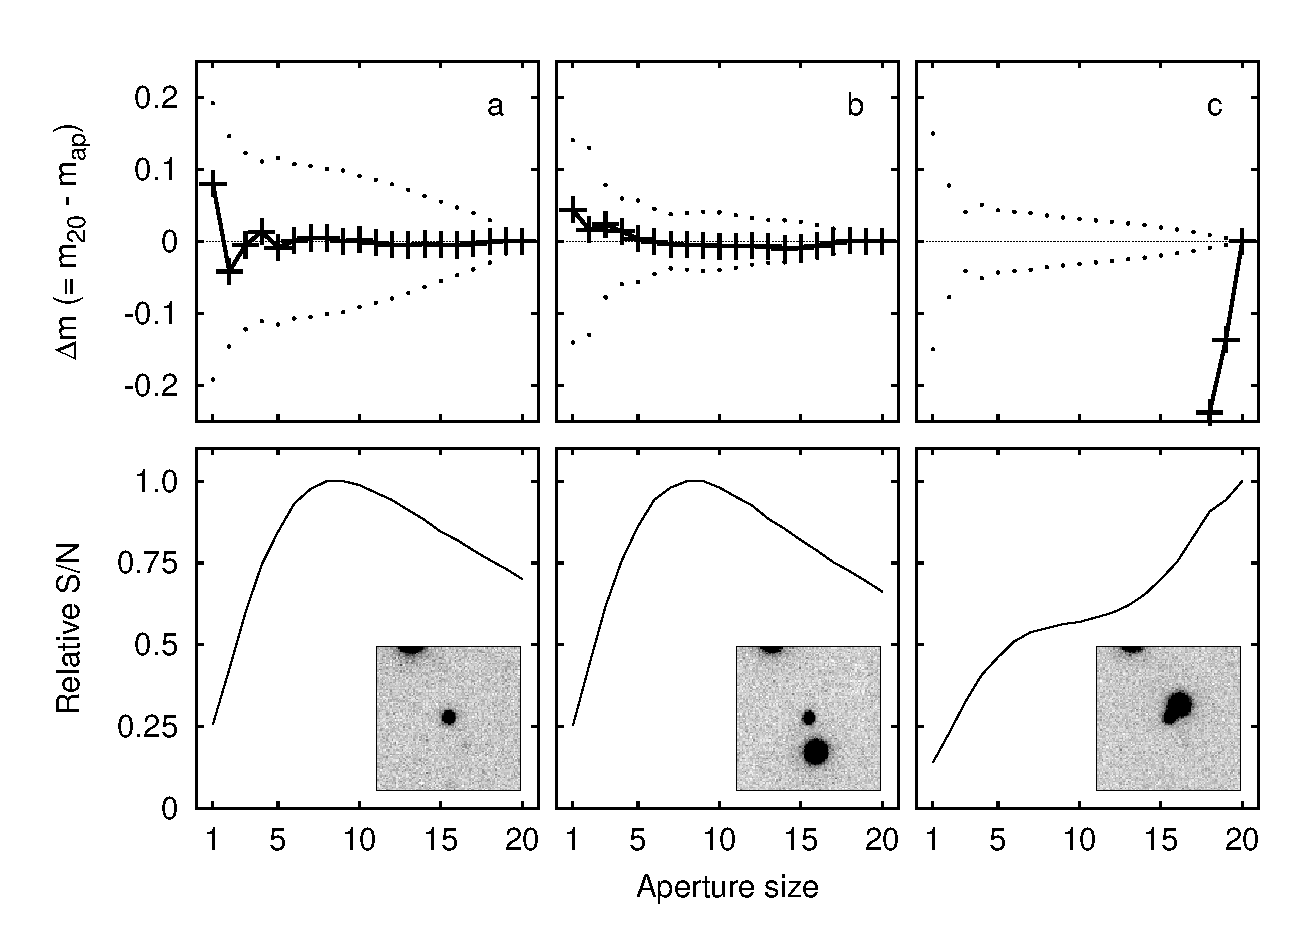
\includegraphics[scale=0.45]{O07_f1.eps}
\caption{Example of multi-aperture indexing method for a star with a passing asteroid.  Differential magnitudes between apertures (solid line) are compared with mean trends for stars of similar brightness (dotted lines), and the difference is indexed.  When there is a signature of contamination (case $c$), different apertures and aperture correction term are automatically applied.}
\end{center}
\label{Fig1}
\end{figure}

\noindent As shown in the Figure 1, we can see whether and at what aperture the differential magnitude of each object begins to deviate from the model curve for each epoch.  It gives us a chance to recover a measurement that otherwise would have been thrown out when the light curve is constructed.  This way, we make a full use of the information offered by the data.  It provides an important role in time-series analysis of the stars suspected to show short-term variability (e.g., flare-like or occultation-like events) because a sudden change of brightness is the main signature that should be disregarded as a measurement failure.  

\subsection{Removal of temporal systematics by photometric de-trending (PDT)}
De-trending is now very familiar term in time-series analysis.  For example, the importance of minimizing known (or unknown) systematics have been recognized by several exo-planet surveys because planet detection performance can be easily damaged by them (e.g., \citealt{kov05, tam05, pon06}).  One interesting property is that {\itshape systematic trends in time-series data can be different and localized within a single CCD frame when the field of view is large}.  This is probably related to subtle PSF (Point Spread Function) differences and sky condition within the detector field of view.  We find that the spatio-temporal characteristics should be considered carefully for wide-field photometry.

In order to reduce temporal systematics in time-series photometry, we use the PDT algorithm that has been designed to detect and remove spatially localized patterns \citep{kim09}.  By default, this algorithm works with a set of light curves that contain the same number of data points distributed in the same series of epoch.  In many cases, however, missing data occur when no photometric measurements are available for some stars in a given observed image.  These missing data can be simply replaced by means, medians, or the values from the interpolation of adjacent data points in each light curve (e.g., \citealt{kov05, kim10}).  Although using the replaced value is the easiest way to reconstruct the light curve to be analyzed, it is not reliable if the time separation between two subsequent observations is too large.  Instead we use more straightforward approach to apply the PDT algorithm in two separate steps: (a) we construct the master trends from the subset of bright stars, and (b) de-trend light curves of all stars with most similar master trend and matching time line.  Here are the main procedure of our de-trending process: \begin{itemize}
\item{We select the template light curves from bright stars.  The length of these light curves should be long enough to cover the entire observing span.}

\item{We extract all subset of light curves that show spatially and temporally correlated features (i.e., clusters).  Each cluster is determined by hierarchical tree clustering algorithm based on the degree of similarity, defined as the Pearson correlation coefficient between the ranks of the light curves.}

\item{We obtain master trends for each cluster, and then de-trend each light curve of all nearby stars by subtracting point-by-point contribution of model trend to the original light curve.}
\end{itemize} 

\begin{figure}[!t]
\begin{center}
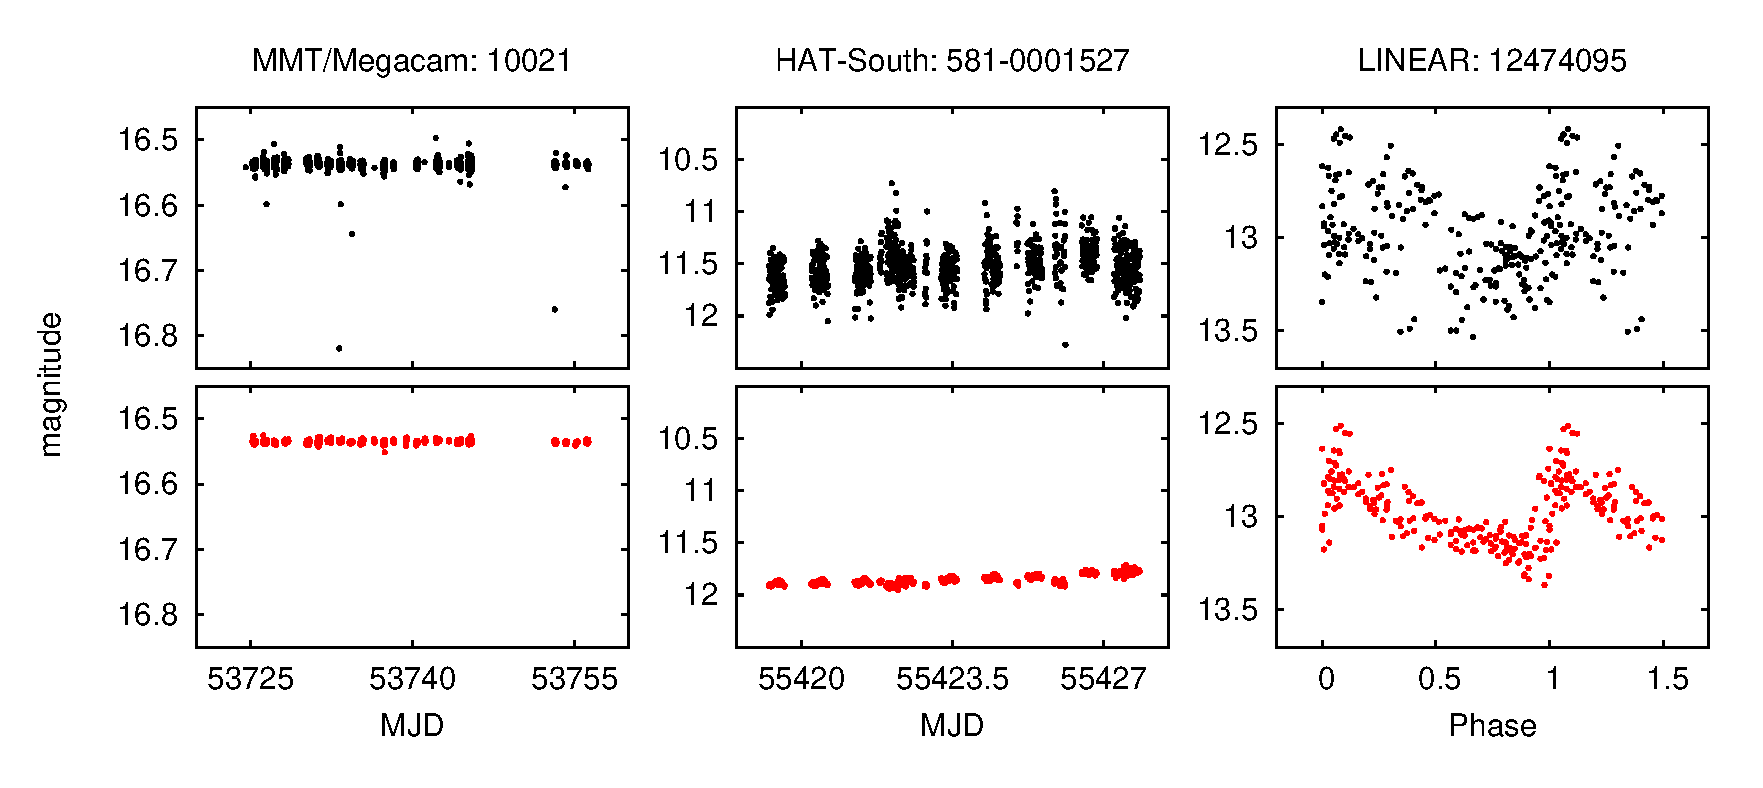
\includegraphics[scale=0.42]{O07_f2.eps}
\caption{Examples of archival or traditionally processed light curves (black) and de-trended light curves (red) for MMT/Megacam, HAT-South, and LINEAR data, respectively.  The last panel exhibits the light curve folded by 0.5228 days (RRab type star).}
\end{center}
\label{Fig2}
\end{figure}

\noindent Figure 2 shows the examples of light curves that bring out the effects of de-trending.  Our method removes serious systematic variations, while true variability is preserved.  As shown in the case of LINEAR, de-trending alone is also a very useful tool in detecting {\itshape real} variable objects that could have been mistaken as a spurious source by greatly reducing systematics from the light curves.

In summary, there is a room to further improve the quality of the astronomical archive data.  Our experiments demonstrate that (a) new calibration can make the old image database useful in finding new variable sources previously not noticed (e.g., MMT/Megacam; HAT-South), and (b) some light curve archives suffer from serious time-dependent biases that can be removed before vigorous variability analysis (e.g., LINEAR).  We want to emphasize the importance of public release of image data obtained in major time-series survey projects.  With rapidly developing computer resources, new and noble re-calibration and analysis methods will allow us to make new discoveries from old survey image archives.  \\

\acknowledgements We thank the MMT/M37 survey and HAT-South research teams for the kind provision of raw image data.  The LINEAR data was gratefully taken from the on-line database SkyDOT.  This research was supported by Basic Science Research Program through the National Research Foundation of Korea (NRF) funded by the Ministry of Education, Science and Technology (2012R1A1A2006924).

%\bibliography{O07}

\begin{thebibliography}{}
\bibitem[Howell(1989)]{how89} Howell, S. B. 1989, \pasp, 101, 616
\bibitem[Kim et al.(2009)]{kim09} Kim, D.-W., Protopapas, P., Alcock, C., Byun, Y. I., \& Bianco, F. 2009, \mnras, 397, 558
\bibitem[Kim et al.(2010)]{kim10} Kim, D.-W., et al. 2010, \aj, 139, 757
\bibitem[Kov\'{a}cs, Bakos, \& Noyes(2005)]{kov05} Kov\'{a}cs, G., Bakos, G., \& Noyes, R. W. 2005, \mnras, 356, 557
\bibitem[Pont, Zucker, \& Queloz(2006)]{pon06} Pont, F., Zucker, S., \& Queloz, D. 2006, \mnras, 373, 231
\bibitem[Tamuz, Mazeh, \& Zucker(2005)]{tam05} Tamuz, O., Mazeh, T., \& Zucker, S. 2005, \mnras, 356, 1466	
\end{thebibliography}

\end{document}